%----------------------->
\subsection{Tipos de SFV}
%----------------------->

\begin{frame}{Tipos de SFV}

Também se faz necessário saber que tipo de SFV está sendo projetado

\vspace{.5cm}

\begin{itemize}
\item Conectado à rede (On-Grid)
\item Autónomo, Isolado ou Independente (Off-Grid)
\end{itemize}

\begin{figure}[H]
	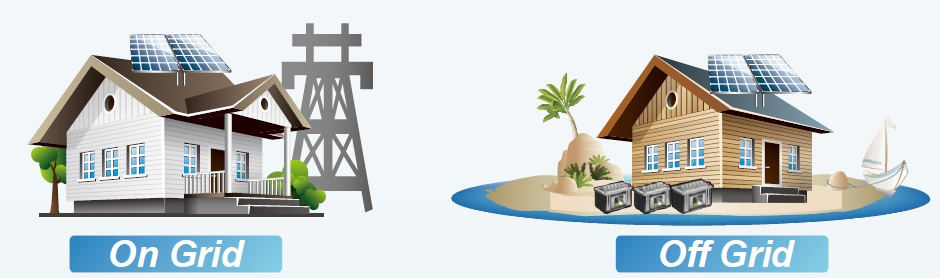
\includegraphics[scale=.4,center]{on-off-grid-solar-power-system}
\end{figure} 

\end{frame}

%----------------------->
\subsection{Componentes}
%----------------------->

\begin{frame}{Componentes dos SFV}

Os SFV são altamente customizáveis, eles podem ser projetados para operar em determinados períodos de tempo ou de acordo com a necessidade de consumo do local.

\begin{center}
    \resizebox{0.6 \linewidth}{!}{%
\begin{tikzpicture}[node distance = 2cm, auto]

\node[Med_block]					(ppv) {Arranjo\\ Fotovoltaico};
\node[Big_esp_block, right=1cm of ppv]	(uccp) {Unidade de Controle\\ e Acondicionamento\\ de Potência};
\node[Med_block, right=1cm of uccp]	(carg) {Carga};
\node[Med_block, above=1cm of carg]	(arma) {Armazena-\\ mento};
\node[Med_block, below=1cm of carg]	(rede) {Rede\\ Elétrica};

\path[line] (ppv) -- (uccp);
\path[line] (uccp) -- (carg);
\path[line] (uccp) -- (arma);
\path[line] (uccp) -- (rede);
 \end{tikzpicture}
    }%
\end{center}
 
\begin{exampleblock}{}
	\begin{center}
	A capacidade para personalizar cada instalação ajuda a minimizar os custos do projeto 
	\end{center} 
\end{exampleblock}
 
 
\end{frame}


\begin{frame}{Componentes dos SFV}

Sistema On-Grid

\begin{center}
    \resizebox{0.9 \linewidth}{!}{%
\begin{tikzpicture}[node distance = 2cm, auto]

\node[Med_block]					(ppv) {Arranjo\\ Fotovoltaico};
\node[Med_esp_block, right=1cm of ppv]	(inv) {Inversor};
\node[Med_esp_block, right=1cm of inv]	(qua) {Quadro de\\ Controle};
\node[Med_block, right=1cm of qua]	(med) {Medição\\ Bidirecional};
\node[Med_block, right=1cm of med](red) {Rede\\ Elétrica};
\node[Med_block, below=1cm of qua](car) {Carga\\ AC};

\path[line] (ppv) -- (inv);
\path[line] (inv) -- (qua);
\path[line] (qua) -- (med);
\path[line] (med) -- (red);
\path[line] (red) -- (med);
\path[line] (qua) -- (car); 
 \end{tikzpicture}
    }%
\end{center}

Sistema Off-Grid

\begin{center}
    \resizebox{0.7 \linewidth}{!}{%
\begin{tikzpicture}[node distance = 2cm, auto]

\node[Med_block]					(ppv) {Arranjo\\ Fotovoltaico};
\node[Med_esp_block, right=1cm of ppv]	(con) {Controlador\\ de Carga};
\node[Med_block, right=1cm of con]	(inv) {Inversor};
\node[Med_block, right=1cm of inv](cca) {Carga\\ CA};
\node[Med_block, below=1cm of con]	(bat) {Bateria};
\node[Med_block, right=1cm of bat](ccc) {Carga\\ CC};

\path[line] (ppv) -- (con);
\path[line] (con) -- (inv);
\path[line] (inv) -- (cca);
\path[line] (con) -- (bat);
\path[line] (con) -- (ccc);
 \end{tikzpicture}
    }%
\end{center}
 
\end{frame}

%%\textbf{Exemplo:} 1.2 kWh/m2/dia (Média anual) obtidos do mapa Solarimétrico para certa localidade.
%%\textbf{Interpretação:} Soma da irradiação de cada dia do ano dividida por 365
